\chapter{TESTING}
\begin{itemize}
\item \textbf {Test Cases (Manual Testing):}
\end{itemize}

\begin{figure}[ht!]
	\centering
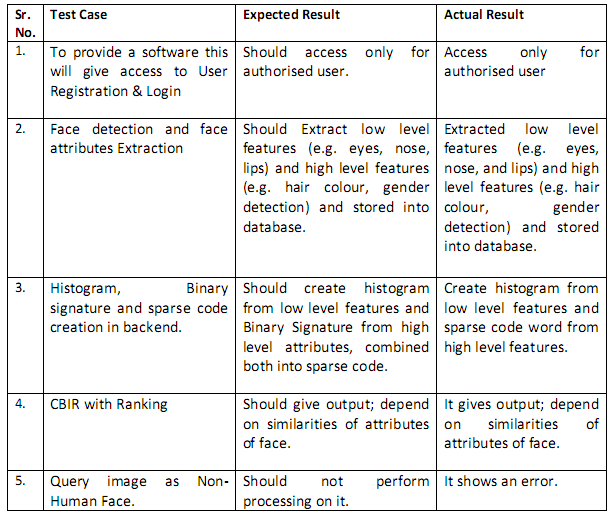
\includegraphics[height=250pt,width=450pt]{test.png}\\
\caption{Test Cases}
\end{figure}
\begin{itemize}
\item \textbf {Testing by Automation Tool:}
\end{itemize}
 We used MERCURY\'s Quick Test Professional 9.2 automation tool for testing our project, we choose this tool because it\’s very efficient for testing and worldwide accepted for testing. QTP can perform following types of testing:\newline\newline\newline\newline
1.	GUI Testing.\newline
2.	Data Driven Testing\newline
3.	Accessibility Testing\newline
4.	Text and Text Area Testing\newline
\textbf{Reasons for choosing QTP for test Automation:}\newline
1.Test Automation framework: From a test framework perspective QTP is one tool that can be used in any type of framework Modular (Record and Playback) driven framework, Data driven (Data tables) Framework (Wow! I love the built in data driver functions and the data driving capabilities of QTP, simply amazing!!!),Keyword driven (Keyword view, function libraries etc.) framework or any other custom framework.\newline
2. Record and Playback: It is pretty easy even for a non-programmer to record scripts / test cases, customize / modify and play back the tests. Also the tool lets the user record the scripts in three different recording modes as per the requirement: Normal, Analog and Low level. Unlike other tools that records every mouse / keyboard events / any java script event on the application, QTP Normal recording mode knows what to record and what not to. The best part is, if you want to record the above said events it can be achieved through the other two recording modes in QTP.\newline
3. Object repository and Object identification process: The Object repository again available in two modes (Shared-For common application objects and Local-For script specific application objects) is personally the best thing I like about QTP. Unlike Test Complete (where a complex object mapping concept is followed), QTP stores the standard and nonstandard properties of the various objects of the AUT (Application under test). At the time of execution, QTP knows exactly where the objects are and how to reach those in a jiffy which increases the efficiency of test execution. The smart processing QTP is definitely a feather on the hat. There is also an ‘object spy’ tool that help you chose the property of an object you can use to automate.\newline
4. In-built function libraries: Quick test professional comes with a huge list of in-built functions (VBScript/QTP) for data manipulation, math, date and time, conversion, string, join and many more functions are available. This ensures that we don’t have to re-invent the wheel, just use it.\newline 
5. Error-Root cause analysis and Recovery: As a tester, I would look for 2 primary things in any application 1: Proper and appropriate error messages 2: Good log reports. Fortunately, Quick Test professional comes with both. Apart from the logs and error messages, we can set break points and find out the values stored in variables at runtime through the full featured Script editor and script debugging features. The recovery scenario manager helps you to recover from any unforeseen events like object state not identified, pop-ups, a statement failure, application crash etc.\newline 
6. Maintenance and Reusability: The idea behind any test automation framework is either Maintainability or Reusability or both. Quick Test professional makes it even easier to maintain the Test Scripts, Functions, objects and everything else built using QTP.\newline
7. Supported environments: Though the tool supports only Windows platform, it can be used for automation in a big list of application platforms but not limited to Java, Oracle, SAP, .NET, Web Forms, Siebel, PeopleSoft, Web services, Main frame (Terminal Emulator), Stingray, Delphi, WPF, Flex, Windows mobiles and not to forget the support for most popular browsers like Internet explorer and fire fox. From the forums, I understand that they are working on support for Google chrome browser. It also supports Rich Internet Applications (RIA) like Ajax, Flex, Silverlight, etc.\newline
8. Support for different testing requirements: Quick Test professional supports any level of testing (Unit, Integration, System, and UAT), regression testing, web application testing, windows application testing, mobile application testing, database, load testing etc. Please read the complete article on QTP supported testing types by clicking on the link.\newline
9. Results viewer: The test run Results viewer furnishes with an executive summary page with data specific to the test , pie charts and statistics for both the current and previous runs, a quick link to the previous run results, and more. It is pretty easy to customize or the set of panes that we can show, hide, move, dock. The best part is the Run results viewer can be installed as a standalone application. This enables us to share the results of the tests with business analysts and developers who do not work with Quick Test professional.\newline
\textbf {We used QTP 9.2 for GUI and Accessibility Testing}

\newpage
\textbf{Snapshot of QTP Testing:}

\begin{figure}[ht!]
	\centering
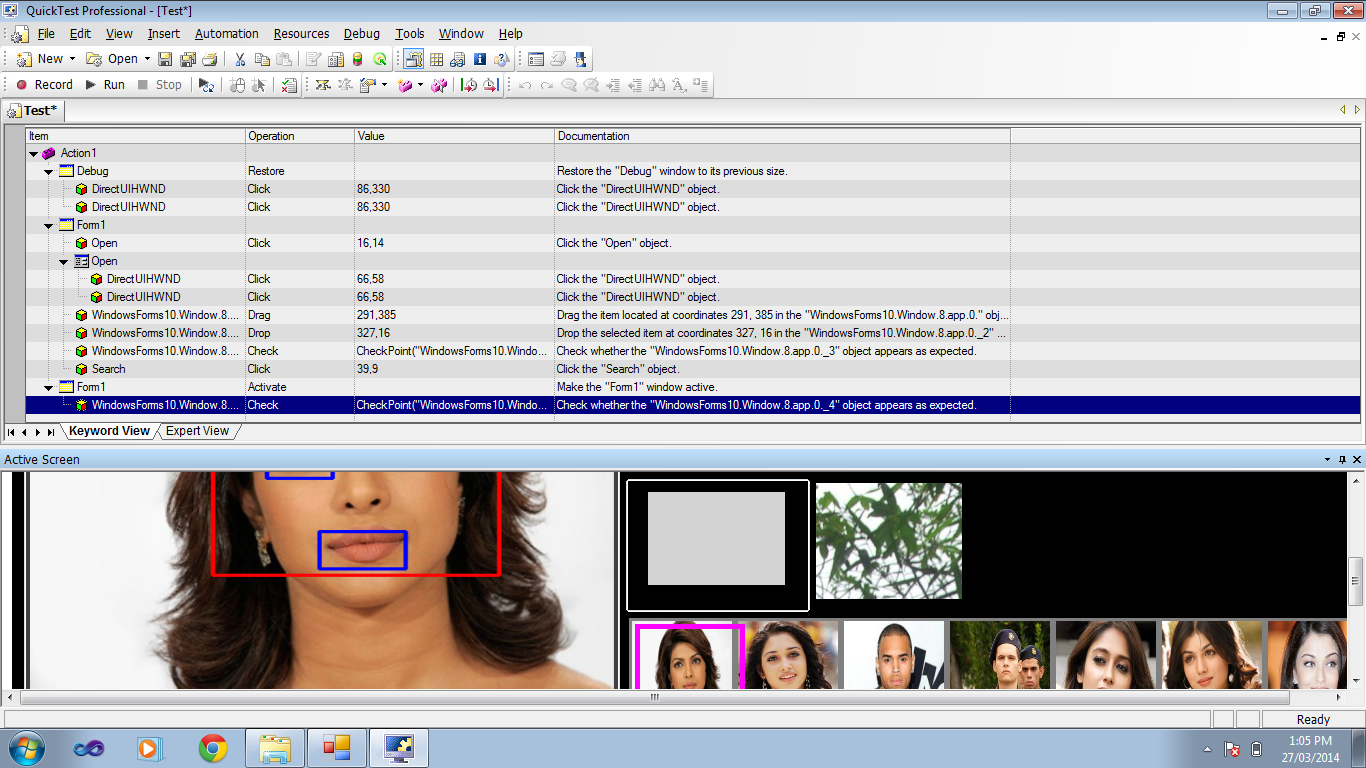
\includegraphics[height=250pt,width=450pt]{qtp1.png}\\
\caption{BitMap Checkpoints in QTP}
\end{figure}

\begin{figure}[ht!]
	\centering
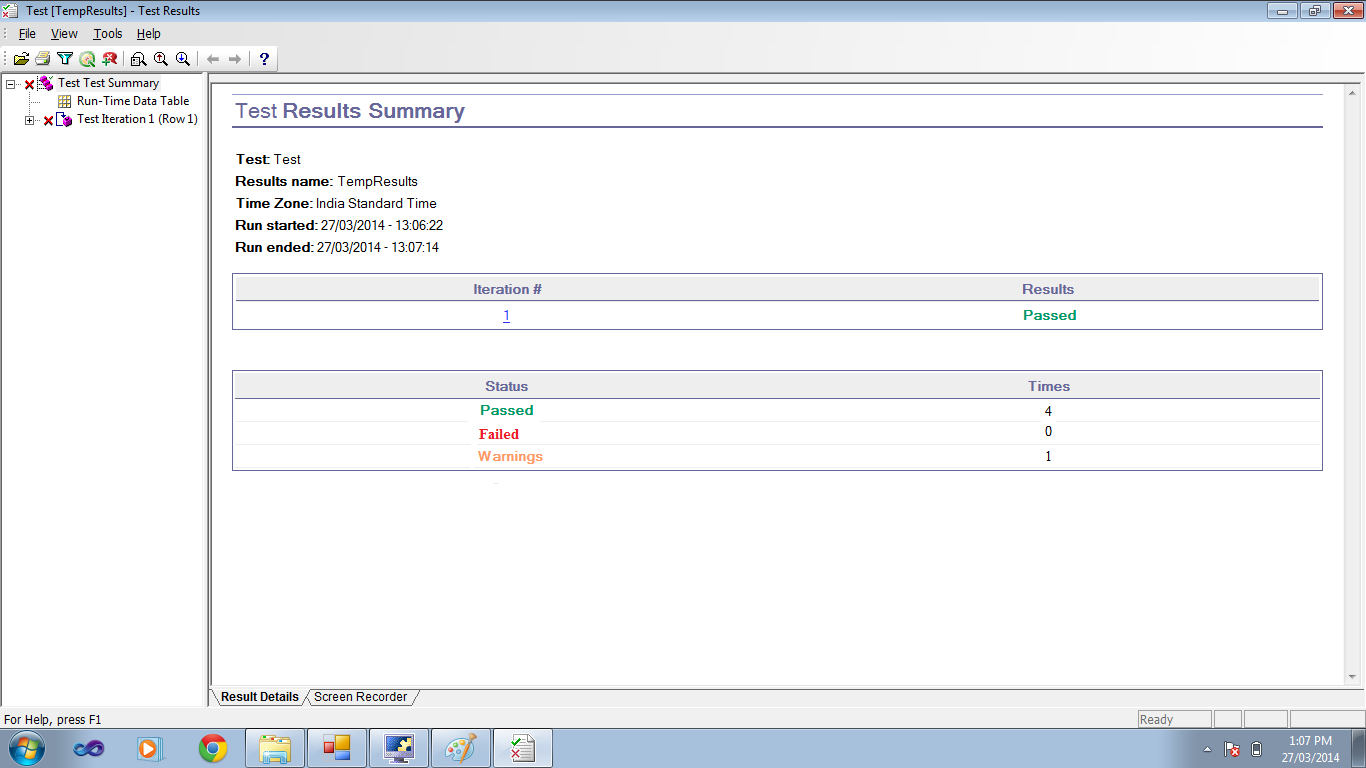
\includegraphics[height=250pt,width=450pt]{test_result.png}\\
\caption{Test Result}
\end{figure}
